\documentclass{article}
\usepackage{full page}
\usepackage{listings}
\usepackage{color}
\usepackage{wrapfig}

\definecolor{mygreen}{rgb}{0,0.6,0}
\definecolor{mygray}{rgb}{0.5,0.5,0.5}
\definecolor{mymauve}{rgb}{0.58,0,0.82}

\lstset{ %
  backgroundcolor=\color{white},   % choose the background color; you must add \usepackage{color} or \usepackage{xcolor}
  breakatwhitespace=false,         % sets if automatic breaks should only happen at whitespace
  breaklines=true,                 % sets automatic line breaking
  captionpos=b,                    % sets the caption-position to bottom
  commentstyle=\color{mygreen},    % comment style
  deletekeywords={...},            % if you want to delete keywords from the given language
  escapeinside={\%*}{*)},          % if you want to add LaTeX within your code
  extendedchars=true,              % lets you use non-ASCII characters; for 8-bits encodings only, does not work with UTF-8
  frame=none,                    % adds a frame around the code
  keepspaces=true,                 % keeps spaces in text, useful for keeping indentation of code (possibly needs columns=flexible)
  keywordstyle=\color{blue},       % keyword style
  language=Java,                 % the language of the code
  morekeywords={*,...},            % if you want to add more keywords to the set
  numbers=none,                    % where to put the line-numbers; possible values are (none, left, right)
  showspaces=false,                % show spaces everywhere adding particular underscores; it overrides 'showstringspaces'
  showstringspaces=false,          % underline spaces within strings only
  showtabs=false,                  % show tabs within strings adding particular underscores
  stringstyle=\color{mymauve},     % string literal style
  tabsize=2,                       % sets default tabsize to 2 spaces
  title=\lstname                   % show the filename of files included with \lstinputlisting; also try caption instead of title
}

\usepackage[pdftex]{graphicx}
\usepackage{float}
\usepackage{caption}
\usepackage{subcaption}
\lstset{language=Java}

\title{Probabilistic Reasoning Over Time}
\author{Michelle Shu}

\begin{document}
\maketitle

\section{Introduction}

In some scenarios, agents are unable to obtain complete information about their environments and must piece together their current state based on experience and partial observations. In this paper, I will describe the application of a probabilistic temporal model to a specific problem of robot localization. 

\vspace{2mm}

The premise of the problem is this: A robot is located at an unknown location on an $n$x$n$ grid. The robot can move in any of the 4 cardinal directions (North, East, South, West), but cannot detect the result of its motion. Thus, if the robot tries to move into a wall, it will not move and stay in its original position, but it has no means of knowing whether it has just moved or not. The robot has only one sensor. It points downward and can tell the robot with better than chance accuracy the color of the grid square beneath it. Using this observation, along with an internal knowledge of both the map and the colors of its grid squares, the robot must infer a probabilistic distribution of its current location.

\section{A Temporal Model for the Blind Robot Problem}

An agent in an unknown environment must keep track what it knows about its current state as it explores the world. Our robot keeps track of a weighted belief state, reflecting the locations where it could possibly be at the current time point and corresponding ratings for its confidence of being in each location (likeliness of being in each location). Using probabilistic inference, the robot modifies its belief state at each discrete time point by following a transition model and a sensor model. The transition model specifies how the robot's location in the world changes with each movement. The sensor model specifies how the color of the floor at a given location is read from the sensor.

\subsection{Transition Model}

I model the changes in the robot's belief state as a first-order Markov process, in which the current belief state (at time $t$) is derived only from the information contained in the previous belief state (time $t-1$), without consideration of the earlier states that occurred before $t-1$. Since the robot's movement is well-defined, it is easy to infer how its belief state will change with each movement. Figure 1 depicts a simple case of a robot on a $2$x$2$ grid. At time $t-1$, the robot believes with some set of probabilities that it is either at location $0$, $1$, $2$ or $3$. We will let $P(L_{t-1} = 0)$ denote what the robot believes to be its probability of being at location $0$ during time $t-1$. Then, after the robot moves, its confidences in its previous locations will shift to adjacent locations in the direction of its movement.

\vspace{2mm}

We don't need to consider the entire realm of possibilities drawn in Fig.1b. In each time step, the robot elects to move one step in a specific direction, so we only need to evaluate the transitions pertaining to a single direction of movement, $m_{t-1}$. In Fig.1c, we assume that the robot has moved North just before time $t$. We use the law of conditional probability on the space of possible transitions given $m_{t-1}$ to compute the values $P(L_t)$ for all grid locations. For example, here is the computation for $P(L_t = 0)$:

\vspace{5mm}

Let $l_{t-1}$ represent all possible locations at time $t-1$.

\vspace{5mm}

$P(L_t=0) = \sum_{l_{t-1}}P(L_t=0 | l_{t-1})P(l_{t-1})$

\vspace{4mm}\hspace{17mm}$ = P(L_t=0 | L_{t-1}=0)P(L_{t-1} = 0) + P(L_t=0 | L_{t-1}=1)P(L_{t-1} = 1)  + $

\vspace{2mm}\hspace{22mm}$ P(L_t=0 | L_{t-1}=2)P(L_{t-1} = 2) + P(L_t=0 | L_{t-1}=3)P(L_{t-1} = 3) $

\vspace{4mm}\hspace{17mm}$ = (1)*P(L_{t-1} = 0) + (0)*P(L_{t-1} = 1) + (1)*P(L_{t-1} = 2) + (0)*P(L_{t-1} = 3) $

\vspace{4mm}$P(L_t=0)=P(L_{t-1} = 0) + P(L_{t-1}=2)$

\vspace{5mm}

As we can see from this derivation, in conjunction with the intuition behind Fig.1c, a probability of $P(L_t = 0)$ is simply the sum of all $P(L_{t-1})$ such that $L_{t-1} + m_{t-1} = 0$ (i.e. moves to position 0). This property generalizes to any location on the grid, hence I use it as the basis for my transition model.

\vspace{5mm}

\begin{figure}[!htb]
\centering
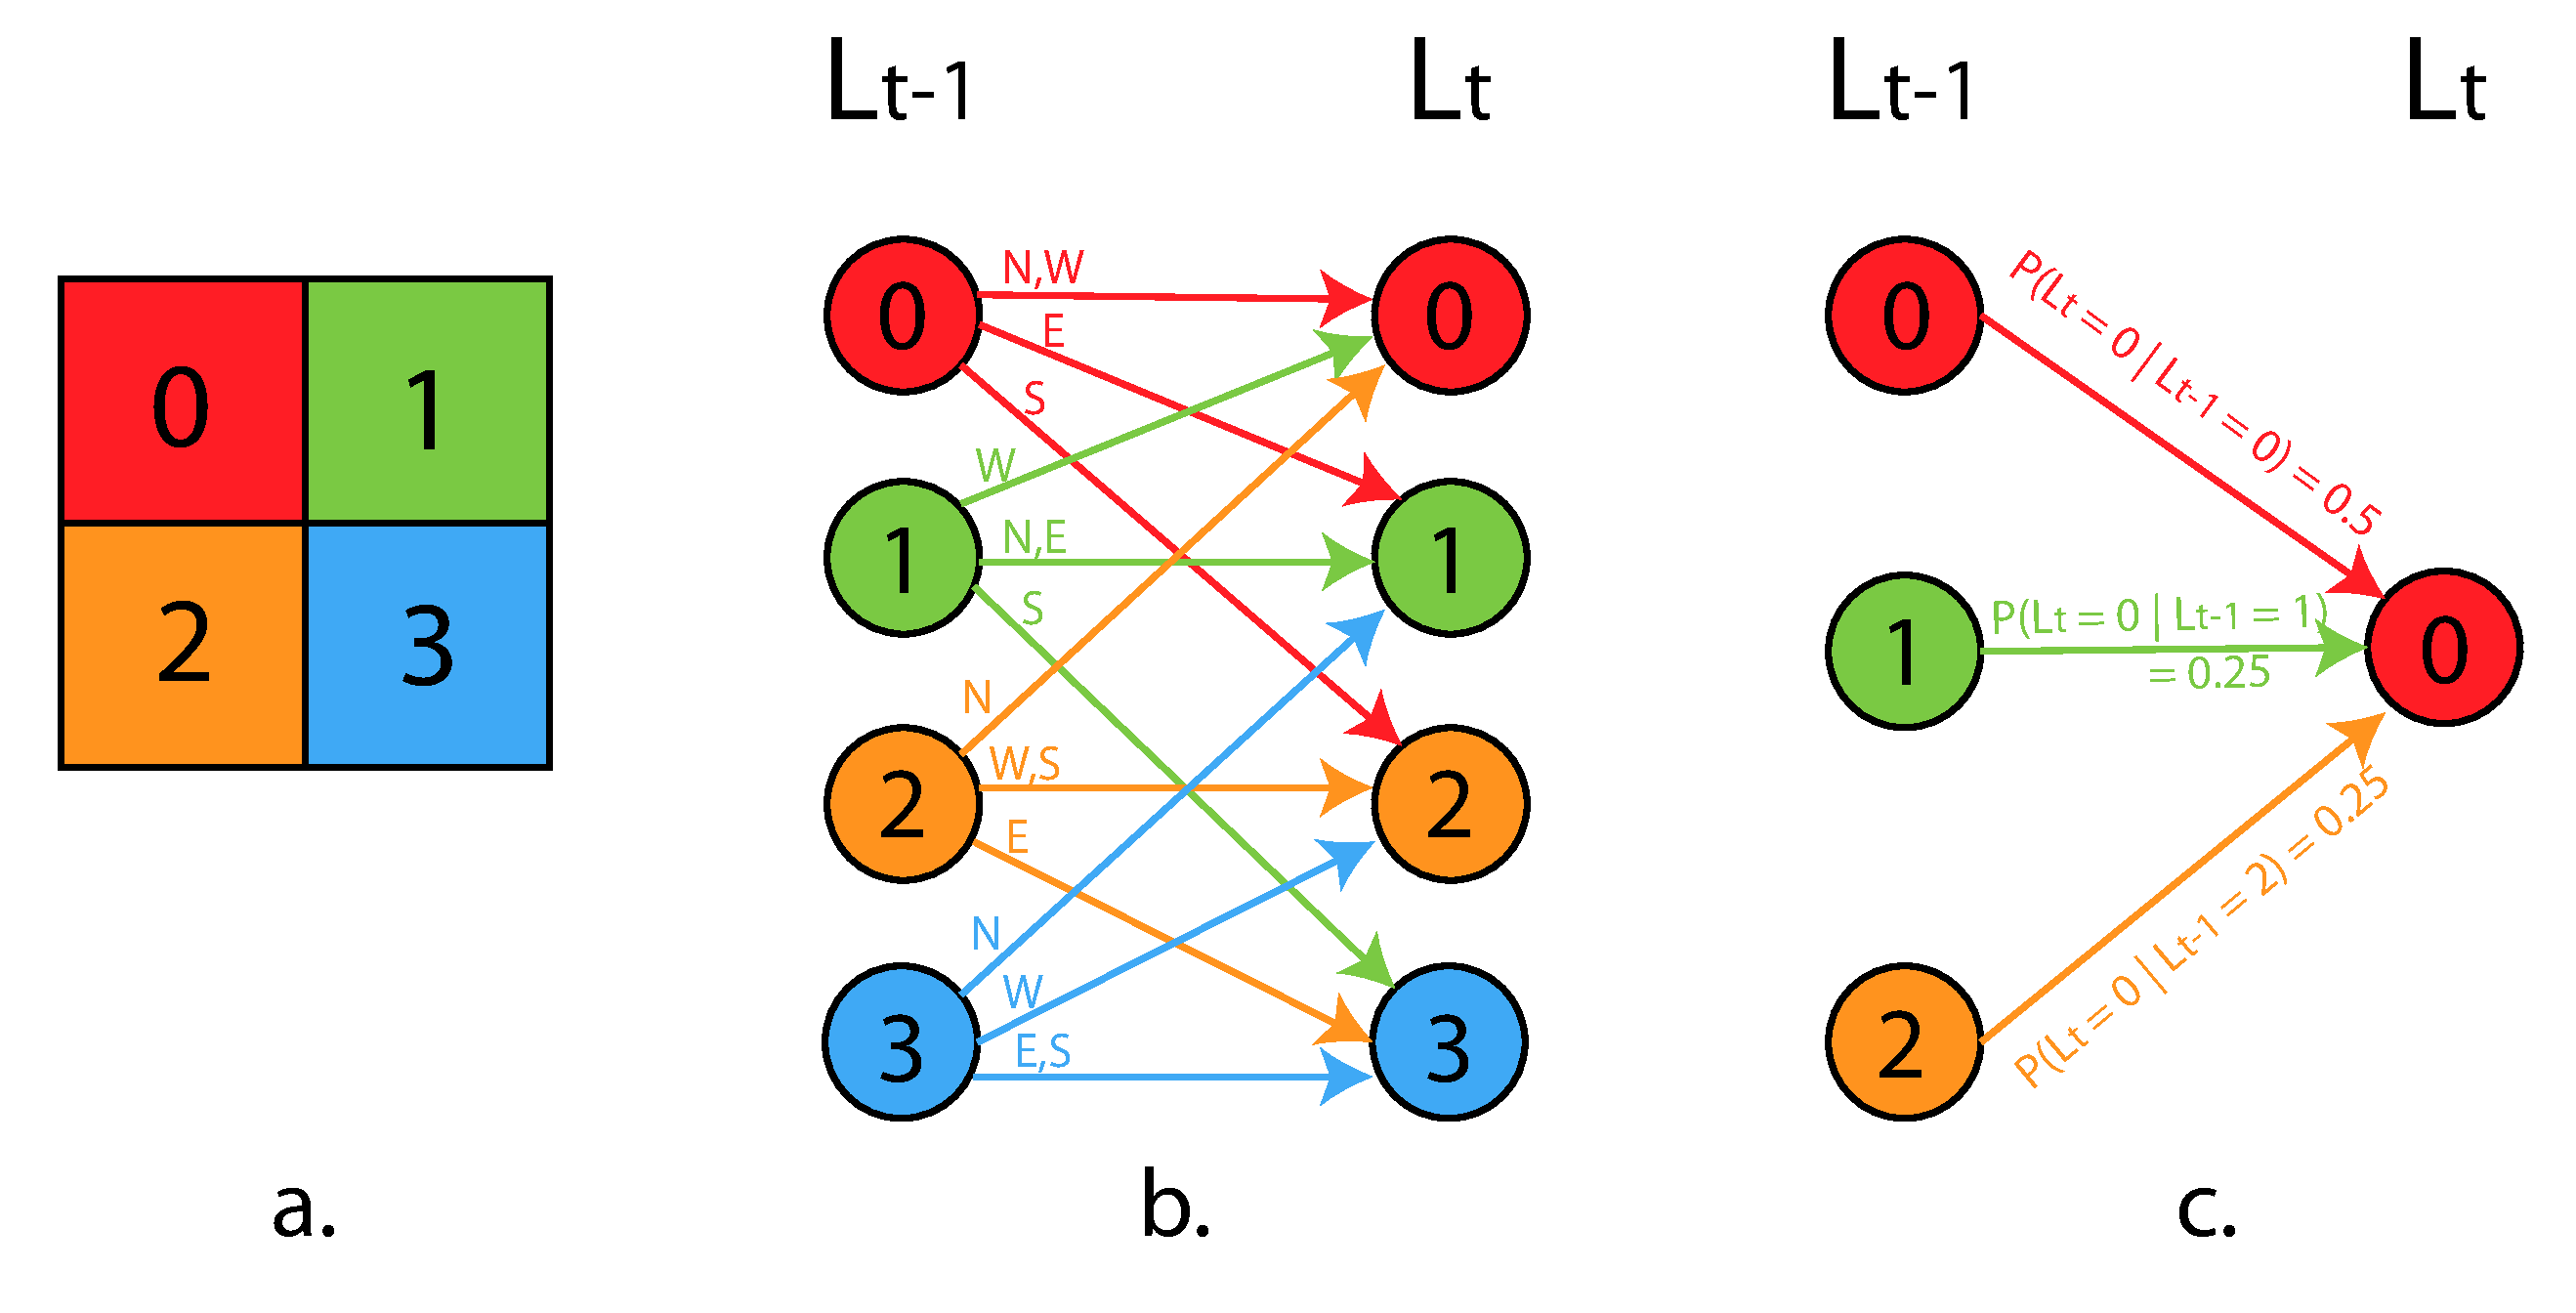
\includegraphics[scale=0.4]{transitions.pdf}
\caption{{\bf State Transition Diagram} a. An example 2 x 2 grid \hspace{2mm} b. All possible state transitions with movements in any of 4 directions \hspace{2mm} c. Provided that the robot moved North, these are possible transitions that would have happened. }
\end{figure}

\subsection{Sensor Model}



\section{Probabilistic Filtering}

One inference technique performed on temporal probabilistic models is called {\bf filtering}. Filtering is the process of computing a belief state based on all evidence and experience gathered up until the current time point. A rational agent will maintain a current state estimate of the probability

\section{Code Design and Implementation}



\end{document}